% This is a sample document using the University of Minnesota, Morris, Computer Science
% Senior Seminar modification of the ACM sig-alternate style. Much of this content is taken
% directly from the ACM sample document illustrating the use of the sig-alternate class. Certain
% parts that we never use have been removed to simplify the example, and a few additional
% components have been added.

% See https://github.com/UMM-CSci/Senior_seminar_templates for more info and to make
% suggestions and corrections.

\documentclass{sig-alternate}
\usepackage{color}
\usepackage[colorinlistoftodos]{todonotes}
\usepackage{amsmath}
\usepackage{subcaption}
%%%%% Uncomment the following line and comment out the previous one
%%%%% to remove all comments
%%%%% NOTE: comments still occupy a line even if invisible;
%%%%% Don't write them as a separate paragraph
%\newcommand{\mycomment}[1]{}

\begin{document}

% --- Author Metadata here ---
%%% REMEMBER TO CHANGE THE SEMESTER AND YEAR AS NEEDED
\conferenceinfo{UMM CSci Senior Seminar Conference, December 2017}{Morris, MN}

\title{Point-of-Interest Recommendation Systems in Location-Based Social Networks}

\numberofauthors{1}

\author{
% The command \alignauthor (no curly braces needed) should
% precede each author name, affiliation/snail-mail address and
% e-mail address. Additionally, tag each line of
% affiliation/address with \affaddr, and tag the
% e-mail address with \email.
\alignauthor
Myeongjae Song\\
	\affaddr{Division of Science and Mathematics}\\
	\affaddr{University of Minnesota, Morris}\\
	\affaddr{Morris, Minnesota, USA 56267}\\
	\email{songx823@morris.umn.edu}
}

\maketitle
\begin{abstract}
Accurate point-of-interest (POI) recommendations are key to the success of 
location-based social networks (LBSN) since it will attract more users and advertisers 
to the platform. To achieve the POI recommendation task, many methods are proposed 
and used in practice from generic recommendation system methods to POI specific 
algorithms. In this paper, we will analyze a novel recommendation technique, 
factorized personalized Markov chain (FPMC) model, which is a combination of matrix 
factorization and Markov chain models. We will also explore enhancements of FPMC 
optimized for POI specific characteristics such as users' movement constraint and 
complex behavior over time. Experimental results show POI specific methods outperform 
generic recommendation models. It also verifies that the more POI characteristics a system incorporates, 
the more accurate the prediction.
\end{abstract}

\keywords{Recommendation Systems, Point-of-Interest Recommendation, Location-Based Social Networks}


\section{Introduction}
\label{sec:introduction}

Nowadays, location-based social networks (LBSN), such as \emph{Facebook places, Tinder},  and \emph{Yelp}, 
have been gaining a lot of attention with the widespread use of smartphones embedded with the 
global positioning system (GPS). Even though LBSNs are relatively new compared to 
the traditional social networking services, millions of active users use the platform on a daily basis voluntarily sharing 
their location information. Many of these LBSNs allow users to ``check-in" to
places like a restaurant or cinema; we call these checked-in places the points of interest (POI) 
of the users. Users can share videos, pictures, or reviews about these places via this ``check-in" 
feature. Based on the collected user data, LBSNs provide POI recommendations. POI recommendation 
is very important for LBSNs for two reasons. First, users are more likely to use the platform and check-in places 
for their own benefit if the quality of recommendation is accurate. 
Second, it allows targeted advertisers to serve specific user groups. Therefore, 
accurate POI recommendation is crucial for the success of LBSNs. \cite{Cheng:2013}

Even though POI recommendation is a type of recommendation system, it has distinct characteristics 
mainly due to its geographical nature. For instance, recommending a movie is a fairly different task from 
recommending a place. A movie recommendation system can recommend any movie, but a POI recommendation 
system should not recommend a sushi restaurant in Tokyo for a user in Minnesota. The following are 
meaningful differences between conventional recommendations and POI recommendation:

\begin{figure}
\centering
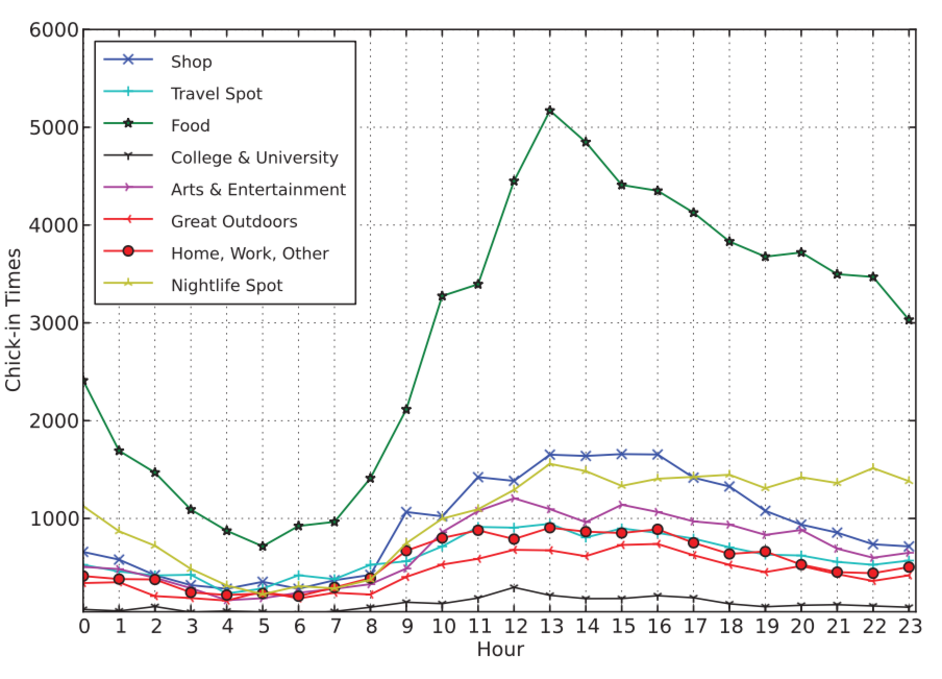
\psfig{file=NYC_checkIn.pdf,width=3.5in}
\caption{Relationship between time interval and check-in location category in NYC. \cite{Li:2017}}
\label{fig:NYC_checkIn}
\end{figure}

\begin{figure*}
\begin{subfigure}{.5\textwidth}
  \centering
  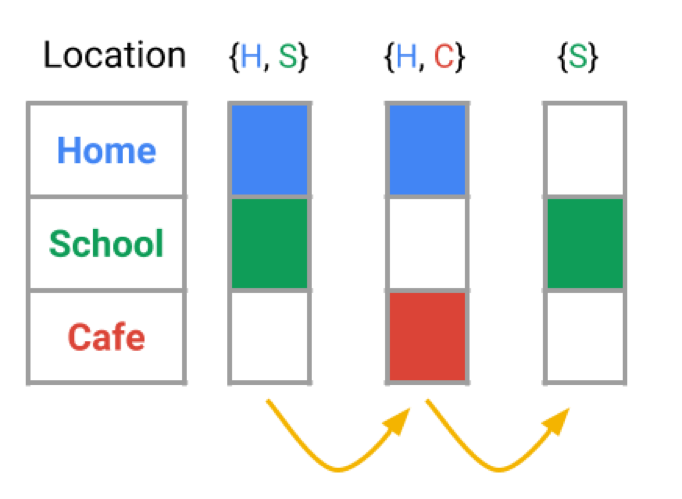
\includegraphics[width=0.75\textwidth]{MCforSets.png}
  \caption{Transition diagram of a Markov chain for sets}
  \label{fig:MCSets}
\end{subfigure}%
\begin{subfigure}{.5\textwidth}
  \centering
  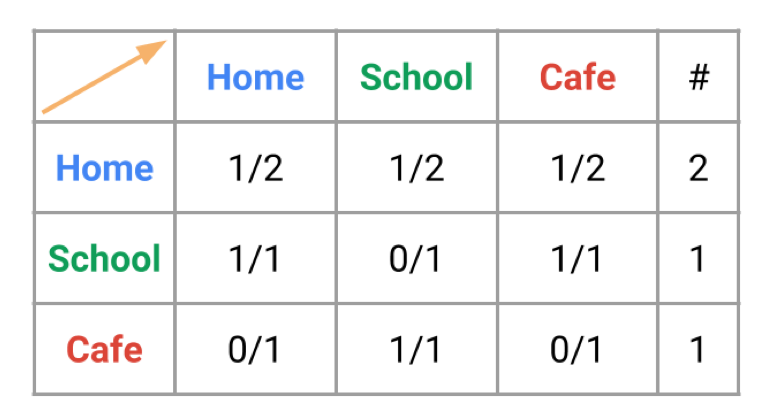
\includegraphics[width=0.75\textwidth]{MCforSetsM.png}
  \caption{Transition matrix for (a)}
  \label{fig:MCSetsM}
\end{subfigure}
\caption{Markov chains for sets}
\label{fig:ex}
\end{figure*}


\begin{itemize}
\item[--] The types of checked-in place are highly related to the time period. Figure \ref{fig:NYC_checkIn} shows check-in data in 
NYC from an LBSN (\emph{Foursquare}) over different hours of a day. The number of check-ins clearly varies depending 
on the time.
\item[--] People are likely to visit nearby places because of geographical limitation. Not many people are willing 
to fly to Japan from the US just for a nice sushi restaurant. \cite{Li:2017}
\item[--] The transition between POIs is strongly affected by the user's own preference. Li et al. \cite{Li:2017} refers to this as a long-term individual preference. For instance, some people go to the gym after work, but some people go home right away after work. 
\item[--] A user's next location is highly related to the user's current location. We would call this the sequential feature of POI recommendations. 
\end{itemize}

\begin{figure*}
\centering
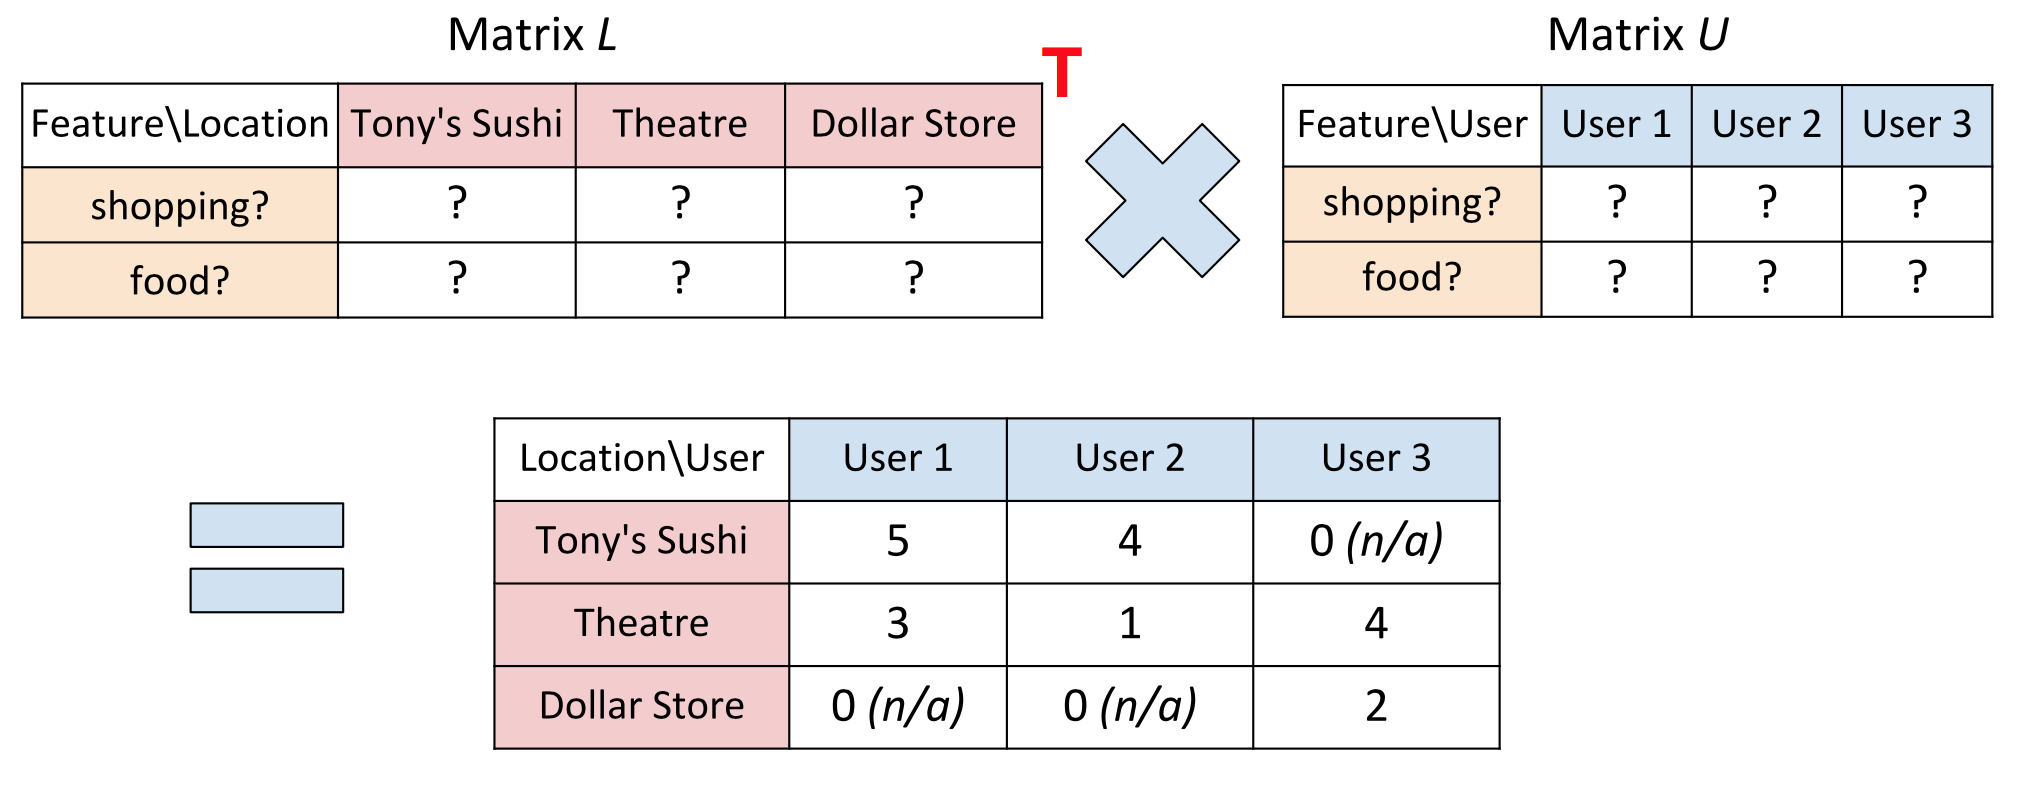
\psfig{file=MF.png,width=6in}
\caption{Matrix factorization of location-user matrix}
\label{fig:MF}
\end{figure*}

Traditionally, matrix factorization (MF) or Markov chains (MC) have been popular techniques for producing recommendations.
The ideas behind MF and MC will be explored in more detail in section \ref{sec:backgrounds}. 
Because of the known drawbacks of each model, Rendle et al. \cite{Rendle:2010:FPM} propose factorized personalized 
Markov chains (FPMC), which is a combination of MC and MF techniques. FPMC is a robust system, 
but it is a generic model and not designed for POI recommendations. To capture the locality feature of 
POI recommendations, Cheng et al. \cite{Cheng:2013} extend FPMC to include localized region (LR) information.  
This extension is abbreviated as FPMC-LR. 
And, Li et al. \cite{Li:2017} propose time-aware FPMC with time decaying consideration called TAD-FPMC.

In section \ref{sec:backgrounds}, we are going to cover mathematical backgrounds in recommendation systems 
to understand the proposed models. Then in section \ref{sec:fpmc}, we will explore the proposed approaches in detail. 
In section \ref{sec:experiments}, we will compare the accuracy of different recommendation techniques: FPMC, FPMC-LR, and TAD-FPMC. 
Finally, we will summarize our findings in section \ref{sec:conclusion}.



\section{Backgrounds}
\label{sec:backgrounds}


\textbf{Markov chain.} Markov chain (MC) is a stochastic process widely adapted in many recommendation systems 
including movie, item, and POI recommendations. An MC is defined on a set of states; each state can be either a value
or a set of values. In the context of LBSN, each state represents a place where users can visit.
Now, we can define an MC as a collection of transitional probabilities among different states.
In other words, it is a map of transitions from one state to another state where transitions are labeled with their probability.  
It is worth pointing out that the sum of all transitions leading out of a state must sum to 1. Another important 
characteristic of the Markov chain is that predictions of future transitions are solely based on the present 
system. Therefore, the previous iterations and future iterations are completely independent. 

When used in location predictions, we often want each state to capture all locations visited over a specific interval of time 
and for our transitions to occur at fixed intervals. This will simplify calculations by allowing us to divide a day into evenly broken hours. 
By expanding our set of states to be non-empty subsets of the set of locations, $L$,  we accomplish this
goal. This new expansion is called Markov chains for sets. Unlike traditional MC, the size of the state space is $2^{|L|}$.
Figure \ref{fig:MCSets} shows an MC for sets. There are three different locations of interest $home$, $cafe$, and $school$. 
These would be the states in a traditional MC model. In an MC for sets, we have 7 non-empty subsets such as $\{home,school\}, \{school\}$, etc.
The extended transition matrix for our expanded set of states rapidly becomes too large to be manageable. 
MC for sets deal with this by estimating a per-location transition matrix that can be used to calculate the probabilities of the extended transition matrix.  
This per-location matrix is estimated using observed transitions. 
Rendle et al. \cite{Rendle:2010:FPM} refer to it as a transition matrix, but it is something a little bit different.

It is easier to understand with an example. 
There are two observed transitions in figure \ref{fig:MCSetsM}: $\{home,school\}$ $\rightarrow$ $\{home,cafe\}$ and 
$\{home,cafe\} \rightarrow \{school\}$.  
Let us call the location associated with a row \emph{start-location} and the location associated with a column \emph{end-location}. 
An entry in our per-location transition matrix is calculated by dividing the number of transitions containing the given \emph{start-location} and 
\emph{end-location}, by the total number of transitions containing the start-location. 
This final number is indicated in \ref{fig:MCSetsM} by the \# column.  
For example, we put a 2 in the column for the row $home$ since 2 transitions start with a set containing $home$. 
This number is then the denominator in all the fractions of the per-location transition matrix. 
There is only 1 transition that has a set containing $home$ that ends in a set containing $school$, 
so the entry for $home \rightarrow school$ is $1/2$.  
This represents the probability that a state containing $home$ will transition to a state containing $school$.

As illustrated in the examples above, we can imagine Markov chains are directly applied to 
POI recommendations but with tens of thousands of places instead of a couple places. Note, in practice, MC based 
approaches use one general transition matrix over all users.

\textbf{Matrix factorization.} In Linear Algebra, matrix factorization (MF) is a technique to 
factor a matrix as a product of multiple matrices. When used in POI recommendation systems, 
the original matrix has two dimensions: locations and users. Consider each row as representing a user and each column 
as representing a location. Each entry in the matrix occurs at a distinct row and column; this entry represents a user's rating 
for that particular location. As you can see in figure \ref{fig:MF}, the final matrix in the figure
has many 0 entries which are the places users have never visited or not rated, so no rating exist. 

Our goal is filling the empty entries by calculating predicted ratings. This is where MF becomes
relevant. By factorizing the location-user matrix, it can be represented as a product of two matrices: 
a location matrix $L$ and a user matrix $U$. Ratings matrix $R$ from figure \ref{fig:MF} is the product of $L$ and $U$:  $R = L U$. 
You might notice that $L$ and $U$ do not have the same dimensionality as $R$. For matrix multiplication to be defined, the number of columns in $L$ and the number of rows in $U$ must match.  
We call this number $f$; it represents the features. In the example, I have chosen  \emph{shopping?} and  \emph{food?} for simplicity, 
but in general the algorithm that does the estimating is given a value for how many features to include and there is not always such a clear-cut way of explaining their meaning. In the diagram, the given number of features is 2. Once we find the two 
factors of $R$, we can make an estimation of unknown ratings. Let $q_l$ be the row associated with location $l$, and 
$p_u \in \mathbb{R}^f$ be the column associated with user $u$. The elements of $q_l$ show how related location $l$ is to its features, 
and the elements of $p_u$ show how interested user $u$ is in the features. If $r_{u,l}$ is the rating of location $l$ 
from user $u$, we can find the estimate rating via multiplying corresponding entries. ~\cite{Koren:2009}
\begin{equation}
	r_{u,l}= q_l p_u
\label{eq:MF}
\end{equation}

The following are some clarifications on the estimation process:
\begin{itemize}
\item[--] The location-user matrix has many missing entries. Thus, the matrix factors ($L$ and $U$ from figure \ref{fig:MF}) are 
estimates whose product produces a matrix similar to the original matrix.
\item[--] The size of $f$ matters with respect to accuracy. If $f$ is too small, we do not 
incorporate enough features for precise predictions. Koren et al. \cite{Koren:2009} verified 
increasing the size of $f$ results in more precise predictions.
\end{itemize}

The factors can be estimated using machine learning techniques.
Rendle et al. \cite{Rendle:2009:BBP} use a technique known as Bayesian personalized ranking (BPR) that attempts 
to produce factors that will be useful for providing a personalized ranking for those locations. 
To apply BPR to Markov chains for sets, sequential BPR (S-BPR) is used. 
The details of BPR and S-BPR are beyond the scope of this paper. For more details see \cite{Rendle:2009:BBP}.

\textbf{Tensor.} From our point of view, a tensor is a multidimensional array in any programming language.
The rank of the tensor is then the number of components needed to specify an entry in the array. 
A vector is a tensor of rank 1 and a scalar is a tensor 
of rank 0. A rank 2 tensor can be represented as a matrix, and higher rank tensors 
are thought of as a multidimensional version of a matrix. For instance, we can stack matrices on 
the top of one another to represent a 3 rank cube-shaped tensor.
Just like matrices can be factorized, tensors can also be factorized. 
This is a key idea of many POI recommendation approaches 
that we will discuss more in the next section.

\begin{figure*}
\centering
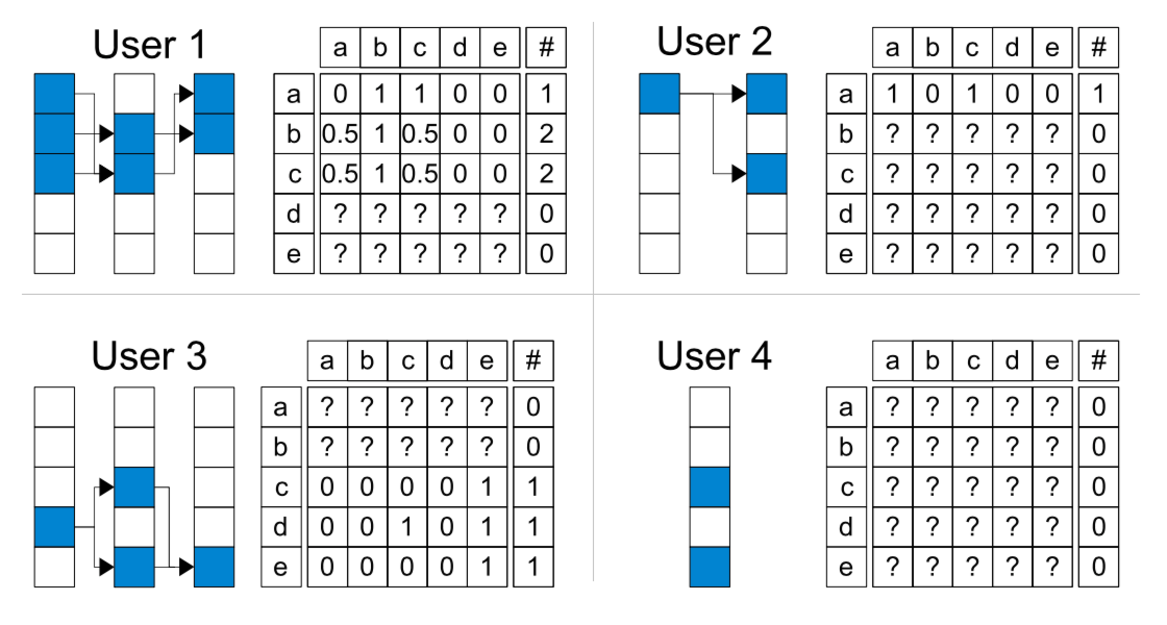
\psfig{file=FPMC_naive.pdf,width = 5in}
\caption{Personalized Markov chains. \cite{Rendle:2010:FPM}}
\label{fig:FPMC_naive}
\end{figure*}

\begin{figure}
\centering
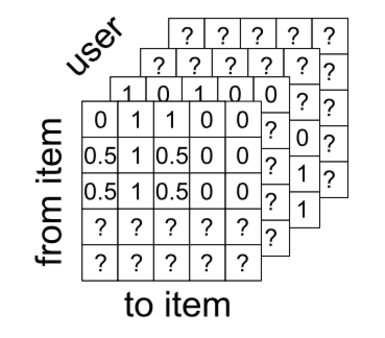
\psfig{file=FPMC.pdf,width= 2in}
\caption{Personalized transition tensor. \cite{Rendle:2010:FPM}}
\label{fig:FPMC}
\end{figure}

\section{Factoring Personalized Markov Chains and its improvements}
\label{sec:fpmc}

As we have discussed in section \ref{sec:backgrounds}, MC and MF based recommendation systems
have fairly distinct characteristics from each other. In this section, we will study a model called 
factorized personalized Markov chain (FPMC) that incorporates MF into MC, and its 
enhancements specializing in LSBN specific data properties.

\subsection{Formalization}
\label{sec:typeChangesSpecialChars}

Before we dive into the details of the algorithms, let us introduce the notation used in this paper. 
Let $U$ be a set of users and $L$ be a set of locations. For each user $u \in U$, 
we know their check-in history set \begin{math}L^t_u\end{math} where $t$ is the interval 
of a user visit. Our goal now is, given the user check-in data 
\begin{math}L^1_u,...,L^{t-1}_u\end{math}, recommend a next location to 
a user $u$ at time $t$. This goal is roughly equivalent to finding the probability of $u$ 
checking in location $l$ at time $t$, given a previous check-in location $i$ at time $t-1$:

\begin{equation}
	x_{u,i,l}=p(l \in L_u^t | i \in L_u^{t-1})
\label{eq:goal}
\end{equation}

\subsection{FPMC}
\label{sec:typeChangesSpecialChars}

Even though MC based recommendation systems were widely studied and used because of 
its capacity to capture sequential data, it lacks the personalization feature to distinguish each user. 
MF also has its weakness in processing sequential information since the order in a user's check-in sequence 
is often ignored when the prediction is calculated.
In section \ref{sec:introduction}, we mentioned sequential information plays a huge role in LBSN 
in that there is a strong connection between users' recently visited locations and future locations. 
Imagine a POI recommendation system with no sequential awareness. 
It may recommend a family restaurant to a user who just checked into a restaurant; this is not ideal. 
To take advantage of these two complementary models, MC and MF, Rendle et al. \cite{Rendle:2010:FPM} propose FPMC.

First, let us think about what kind of recommendation model we aim to build. 
We want a recommendation system that is aware of sequential pattern and personalized for each user.
MC is good at recognizing sequential features, but it uses one general transition matrix for every user. 
Then, the question is, can we create a personalized MC?
A straightforward approach is having a personalized MC per user $u \in U$. 
Figure \ref{fig:FPMC_naive} shows four different transition matrices for each user. 
The question mark (?) entries mean we have no data to estimate the probability of the transition. The problem of these personalized 
MC matrices is that they are often very sparse, so they result in poor estimations. We just do not have enough data from
each user. This is the place where the ideas of MF can be applied. By stacking all transition matrices of users, 
we can get a transition cube or tensor $\chi$. Now, we can factorize the tensor using a tensor factorization technique. 
Factorizing this tensor $\chi$ produces four parameters: one rank-3 core tensor and three matrices. Using an efficient tensor 
factorization technique pairwise interaction tensor factorization (PITF), we get the following 
estimation equation for the probability of user $u$ going to location $l$ from location $i$. \cite{Rendle:2010:PIT}

\begin{equation}
	\hat{x}_{u,i,l} := \underbrace{v_u^{U,L} \cdot v_l^{L,U}}_{A} + \underbrace{v_l^{L,I} \cdot v_i^{I,L}}_{B} 
	+ \underbrace{v_u^{U,I} \cdot v_i^{I,U}}_{C}
\label{eq:FPMC}
\end{equation}

\begin{itemize}
\item[--] A: Interaction between the user features $v_u^{U,L}$ and the next location $v_l^{L,U}$.
\item[--] B: Interaction between the current location $v_l^{L,I}$ and the next location $v_i^{I,L}$.
\item[--] C: Interaction between the user features $v_u^{U,I}$ and the current location $v_i^{I,U}$.
\end{itemize}

This is the essence of the FPMC method. To achieve the recommendation goal $\hat{x}_{u,i,l}$, we 
construct a tensor containing MCs for users, and then we factorize the tensor into a rank-3 tensor 
and matrices. Finally, we calculate the prediction by combining the corresponding entries of the
factors. 

\subsection{FPMC-LR}
\label{sec:typeChangesSpecialChars}

FPMC successfully constructs a personalized MC model for POI recommendation
by combining ideas of MF and MC. However, it overlooks another noticeable property 
of an LBSN dataset, localized region constraint. According to check-in data from 
\emph{Gowalla} and \emph{Foursquare}, more than 75\% of check-ins from Foursquare and 80\% of check-ins 
from Gowalla happened within 10 km of the previously checked-in place. \cite{Cheng:2013} The observation on the LBSN data
shows the trend that users tend to check in places close to their previous check-ins, 
but FPMC does not really make use of this potentially useful trend.

To add the ability to use localized region constraint 
information into the existing FPMC model, Cheng et al. \cite{Cheng:2013}
introduces FPMC-LR which combines the FPMC model with localized 
region (LR) constraints to provide accurate successive POI recommendation in LBSNs. 
Because FPMC-LR only takes into account nearby candidate locations depending 
on where the users currently are, it reduces the computational costs and noisy information. 
Also, it results in more accurate predictions as we will see in section \ref{sec:experiments}.

FPMC-LR has a similar setting to FPMC since it is an improvement 
over FPMC. Just like FPMC, the fundamental goal of FPMC-LR is to give the most suitable 
location recommendation for user $u$ at time $t$ given a sequence of check-in data. 
In other words, we need to calculate $x_{u,i,l}$, which is the probability of a user $u$ visiting a location $l$ at time $t$,
where $i$ is the user location at time $t-1$.
The main difference between FPMC and FPMC-LR is in their transition tensor. As we saw earlier, FPMC takes into account 
all possible locations for each user, so the tensor looks like this: 
\begin{equation}
	\chi \in [0, 1]^{|U| \times |L| \times |L|}
\label{eq:summation}
\end{equation}
Unlike FPMC, FPMC-LR only considers neighborhood locations of the previous check-in location $i$. 
The tensor transition in FPMC-LR looks like this:
\begin{equation}
	\chi \in [0, 1]^{|U| \times |L| \times |N_d(L)|}
\label{eq:summation}
\end{equation}
The set of neighborhood locations \begin{math}N_d(L)\end{math} is calculated by the Haversine formula, 
which is used to find the shortest distance between two points on the surface of a sphere. 
In this case, we assume the earth is roughly a sphere. By applying the same tensor factorizing technique PITF to 
our tensor $\chi \in [0, 1]^{|U| \times |L| \times |N_d(L)|}$, we can calculate the target probability $x_{u,i,l}$.

\subsection{TAD-FPMC}
\label{sec:typeChangesSpecialChars}

FPMC-LR is a successful model for POI recommendation in terms of performance and efficiency 
as we will discuss in section \ref{sec:experiments}; it incorporates sequential data with personalization and locality consideration. 
However, there is still room for improvement. Li et al. \cite{Li:2017} point out that the FPMC-LR approach simply captures 
the consecutive ordering relations in lieu of considering complex user behavior over time. Take college students, 
for example. Students have morning classes, afternoon classes, or both in one day. When they have morning classes, 
some of them have breakfast at a brunch cafe after class. When they have afternoon classes, some of them go 
for a drink at a bar after class. Simply combining them as one sequential pattern is clearly not sufficient (e.g. recommending a bar after an 8:00AM class). In other words, just recognizing sequential data is not 
enough for capturing the differences in regular periodic pattern.

To make the system aware of users' time-varying behavioral trends, Li et al. \cite{Li:2017} suggest the time-aware FPMC (TA-FPMC) 
model, which is an improvement over the FPMC-LR model. Both FPMC and FPMC-LR use a third order tensor to 
construct a personalized Markov chain. TA-FPMC takes a similar approach but one step forward. Instead of a third order tensor of 
user-location-location, it forms a fourth order tensor user-time-location-location by adding a time factor. Our transition tensor looks like this: 
\begin{equation}
	\chi \in [0, 1]^{|U| \times |T| \times |L| \times |L|}
\label{eq:TA-FPMC_tensor}
\end{equation}

Using the tensor factorization technique PITF that we used earlier for FPMC and FPMC-LR, we get 
one rank-3 core tensor and six matrices which capture the following interactions similar to equation \ref{eq:FPMC}.

\begin{itemize}
\item[--] A: Interaction between the user features $v_u^{U,T}$ and the time period $v_t^{T,U}$.
\item[--] B: Interaction between the user features $v_u^{U,I}$ and the current location $v_i^{I,U}$.
\item[--] C: Interaction between the user features $v_u^{U,L}$ and the next location $v_l^{L,U}$.
\item[--] D: Interaction between the time period $v_t^{T,I}$ and the current location $v_i^{I,T}$.
\item[--] E: Interaction between the time period $v_t^{T,L}$ and the next location $v_l^{L,T}$.
\item[--] F: Interaction between the current location $v_i^{I,L}$ and the next location $v_l^{L,I}$.
\end{itemize}

By adding up the corresponding entries in interaction matrices, we get our target value $x_{u,t,i,l}$
\begin{equation}
\begin{split}
\hat{x}_{u,t,i,l} := \underbrace{v_u^{U,T} \cdot v_t^{T,U}}_{A} + \underbrace{v_u^{U,I} \cdot v_i^{I,U}}_{B} + 
								\underbrace{v_u^{U,L} \cdot v_l^{L,U}}_{C}  \\
	                        + \underbrace{v_t^{T,I} \cdot v_i^{I,T}}_{D} + \underbrace{v_t^{T,L} \cdot v_l^{L,T}}_{E} + 
	                        \underbrace{v_i^{I,L} \cdot v_l^{L,I}}_{F}
\end{split}
\label{eq:TAD-FPMC}
\end{equation}

There is another statistical characteristic of LBSN data that has not gotten much attention, the time gap between 
two successive check-ins. The LBSN data shows that many of two successive check-ins span a large time gap 
like a year. Base on the assumption that these successive check-ins with large time gaps do not tell much, 
Li et al. \cite{Li:2017} introduce another factor $D(\Delta t)$ to take into account the time-decaying effect. 
The final model with all the considerations is called TAD-FPMC. There are a few variations of TAD-FPMC that 
are highly optimized for certain data, but we focus on the most basic model of TAD-FPMC for simplicity. 
For more information about TAD-FPMC, refer to \cite{Li:2017}.

\begin{figure}
\centering
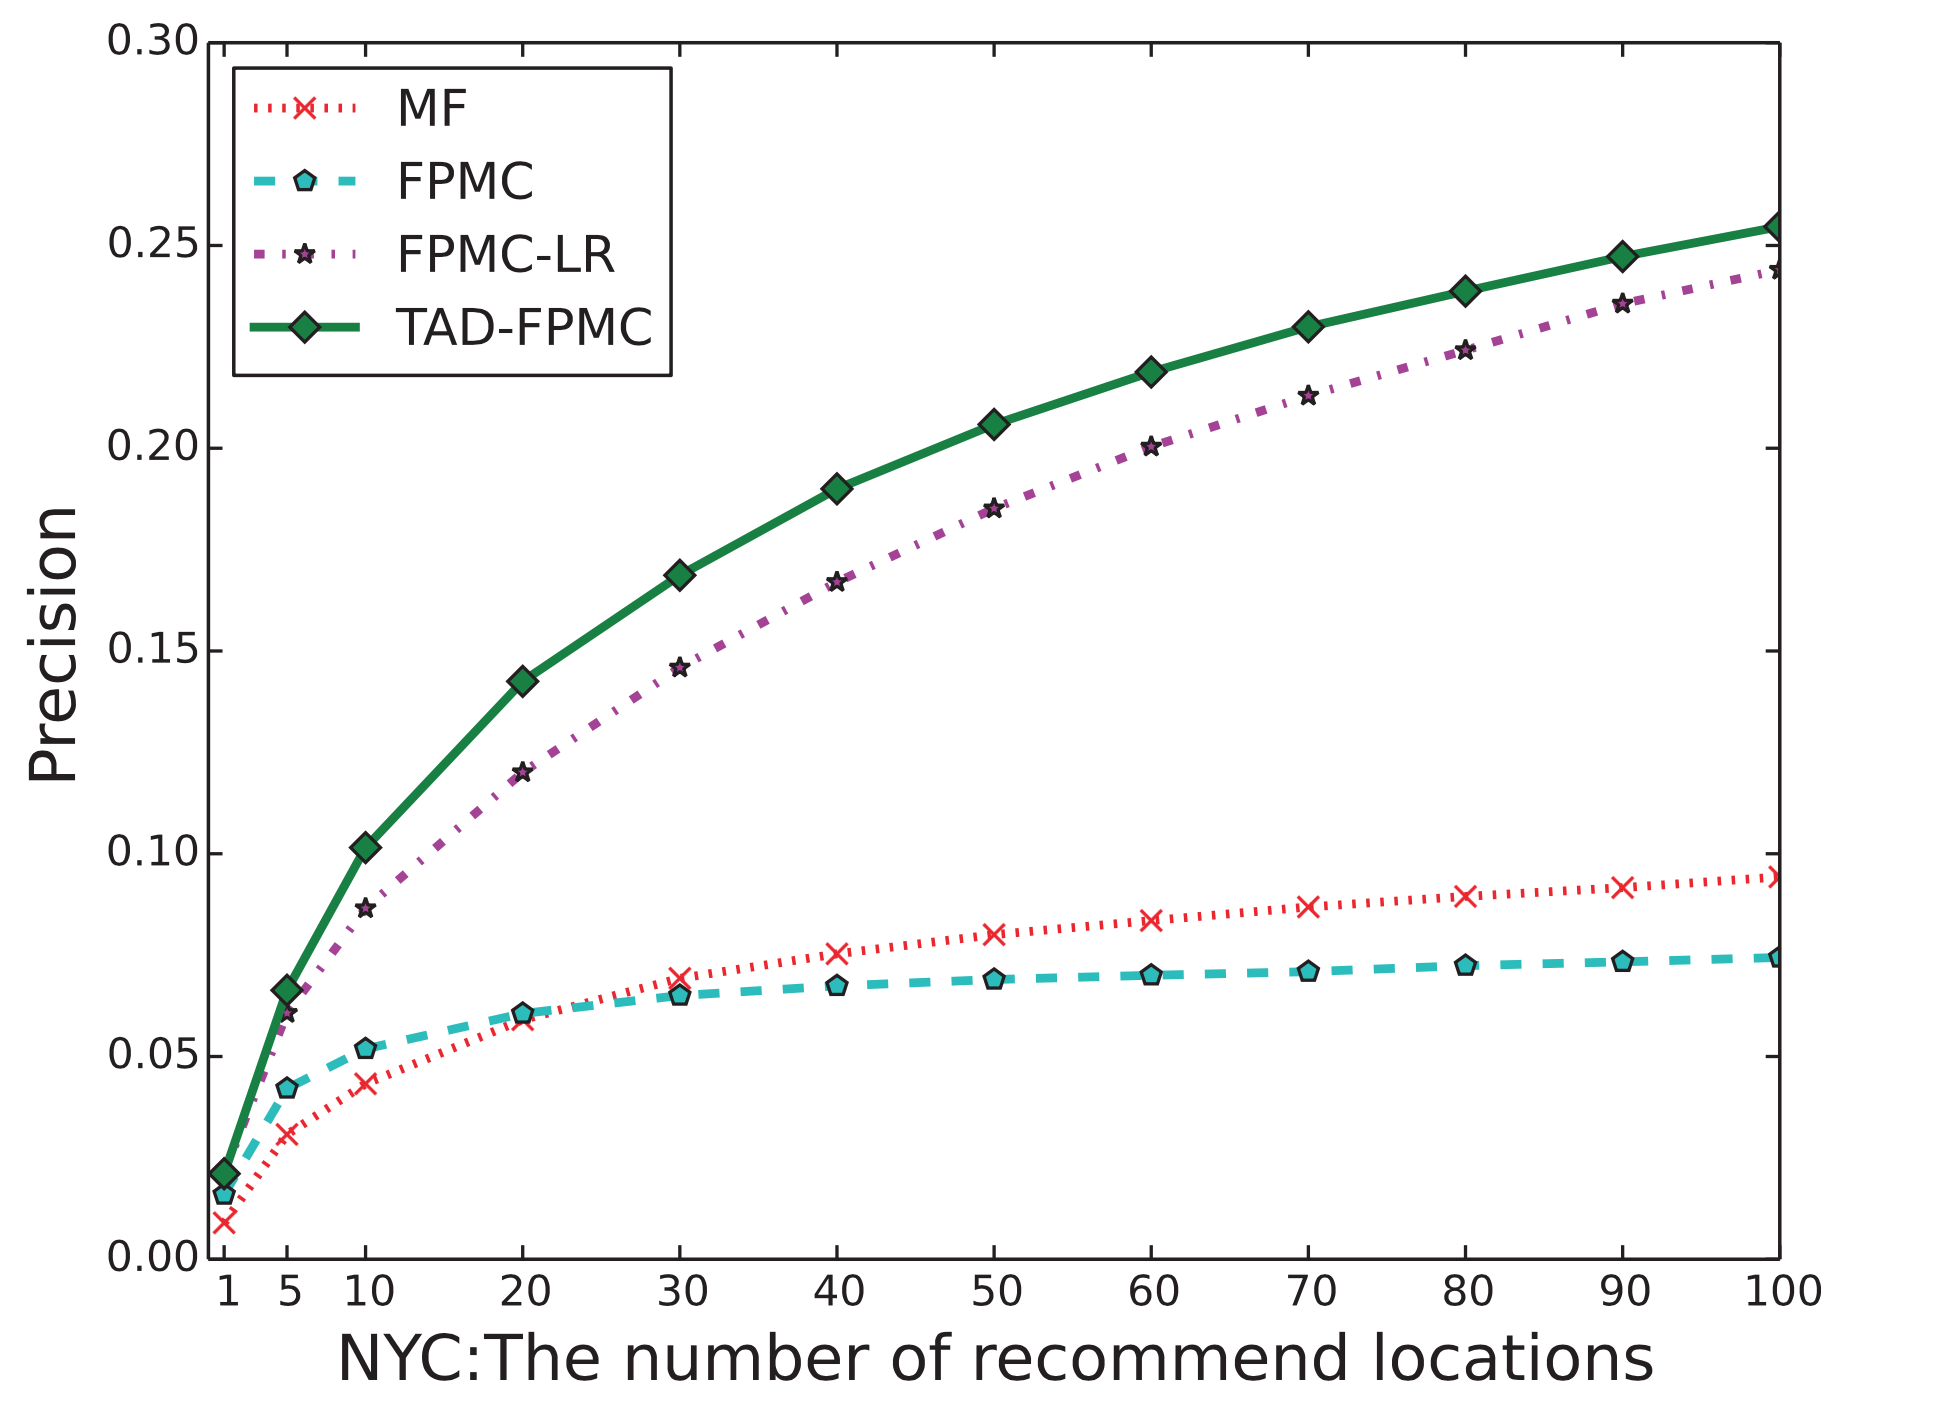
\psfig{file=NYC_ex.png,width= 3.5in}
\caption{Comparison of location prediction in NYC \cite{Li:2017}}
\label{fig:ex_NYC}
\end{figure}

\section{Experiments}
\label{sec:experiments}
In this section, we will address the following questions: 1) How do different POI recommendation 
models perform in real LBSN data? 2) Why are distance constraint and temporal information particularly important 
in the POI recommendation?

\subsection{Datasets}
\label{sec:datasets}
The evaluation used data collected from Foursquare, an LBSN that provides POI recommendations. 
The data includes users' check-in data for New York City from Jan. 
2010 to June 2011. The statistics of data is summarized in table \ref{tab:stat}. \cite{Li:2017}

\begin{table}[ht]
\centering
\caption{The Statistics of Data \cite{Li:2017}}
\bigskip
\label{tab:stat}
\begin{tabular}{|c|c|c|c|}
        \hline
        City & User & Location & Category \\
        \hline
        New York City & 2,581 & 206,416 & 249 \\
        \hline
\end{tabular}
\end{table}

\subsection{Evaluation Metric}
\label{metic}
The main task for the algorithms is providing a list of the top-N recommended locations
ordered from the highest probability of user visit to the lowest. Evaluation metrics take advantage of historic data.  
A location recommendation is considered correct if the user had visited that place in the past. 
The evaluation metric $P@N$ (Precision) is defined as:
\begin{equation}
	P@N = \frac{\textrm{the counts of correct predictions}} {\textrm{the total number of recommendation rounds}}
\label{eq:P@N}
\end{equation}
The number of recommendation rounds is a constant representing the number of times a top-N list was 
generated and checked if correct.

\subsection{Comparison}
\label{comparison}
Figure \ref{fig:ex_NYC} shows the performance comparison among different algorithms of POI recommendation. 
The x-axis represents the number of recommended locations, $N$, and the y-axis 
is the precision of the recommendation $P@N$. In the graph, there is a huge gap 
between generic models (MF and FPMC) and POI specific models (FPMC-LR and TAD-FPMC). 
This verifies the importance of distance constraint and temporal information in POI recommendations. 
Also, TAD-FPMC slightly outperforms FPMC-LR in both datasets. More sophisticated variations of TAD-FPMC outperform 
all the models examined in this paper. The curious reader is referred to \cite{Li:2017}.
The experiments were run on a quad-core machine with a Core i7-6700K 4.0GHz 8 hyper-threading and memory size of 32GB. \cite{Li:2017} 

\section{Conclusion}
\label{sec:conclusion}

In this paper, we have considered the point-of-interest (POI) recommendation in LBSNs 
and introduced different approaches for accurate predictions. Factorized personalized Markov 
chain (FPMC) model is an elegant method combining advantages of Markov chains and matrix factorization,
but it was not designed to incorporate distinct characteristics of LBSN data. FPMC-LR is an enhancement 
of FPMC by only considering nearby locations when calculating POI predictions. TAD-FPMC is a novel 
POI recommendation system approach that captures complex user behavior over time in addition to inheriting strengths 
of FPMC and FPMC-LR models. From experimental results conducted on Foursquare data for LA and NYC, we conclude 
POI recommendation specific approaches (FPMC-LR, TAD-FPMC) far outperform generic recommendation models such as FPMC.
Additionally, TAD-FPMC produces better predictions than any other methods including FPMC-LR.


\section*{Acknowledgments}
\label{sec:acknowledgments}

I thank my senior seminar professors, Peter Dolan and Kristin Lamberty, 
for their helpful advice and comments throughout the research and writing process.

% The following two commands are all you need in the
% initial runs of your .tex file to
% produce the bibliography for the citations in your paper.
\bibliographystyle{abbrv}
% sample_paper.bib is the name of the BibTex file containing the
% bibliography entries. Note that you *don't* include the .bib ending here.

\bibliography{sample_paper}  
% You must have a proper ".bib" file
%  and remember to run:
% latex bibtex latex latex
% to resolve all references

\end{document}
